\section{TEST A-CLUS BASE}

Durante la fase di testing, sono stati analizzati diversi scenari critici per validare la robustezza dell'applicazione:

\subsection{Gestione di tabelle inesistenti}

\begin{figure}[h!]
    \centering
    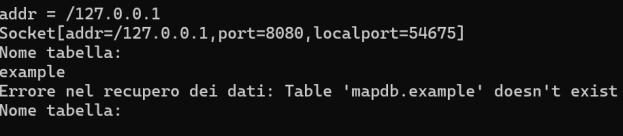
\includegraphics[width=\textwidth]{images/errore_tabella.png}
\end{figure}

Quando viene specificato un identificativo di tabella non presente nel database, il sistema visualizza un appropriato messaggio diagnostico e offre all'utente la possibilità di inserire una denominazione alternativa.


\subsection{Validazione delle selezioni di menù}

La schermata di selezione del menù principale consente di scegliere tra due opzioni: "Carica Dendrogramma" o "Esegui Clustering".

\begin{figure}[h!]
    \centering
    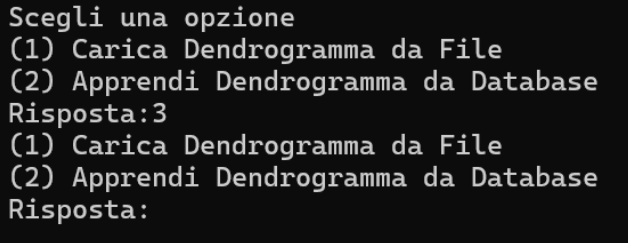
\includegraphics[width=\textwidth]{images/errore_men.png}
\end{figure}

L'inserimento di valori non conformi alle opzioni disponibili (diversi da 1 o 2) viene intercettato, consentendo all'utente di ripetere la selezione senza interruzioni del flusso operativo.

\subsubsection{Controllo sull'esistenza degli archivi} 
\begin{figure}[h!]
    \centering
    \includegraphics[width=\textwidth]{images/controllo_archivi.png}
\end{figure}
Nel caso di caricamento di un dendrogramma precedentemente salvato, il sistema verifica l'esistenza dell'archivio specificato. In caso negativo, viene presentata una notifica e l'applicazione termina la sessione.

\subsubsection{Validazione parametri di profondità} 
    \begin{figure}[h!]
        \centering
        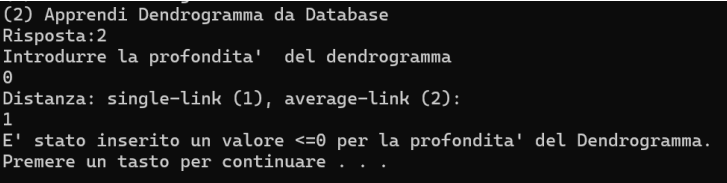
\includegraphics[width=\textwidth]{images/0_valore_errato.png}
    \end{figure}

    \begin{figure}[h!]
        \centering
        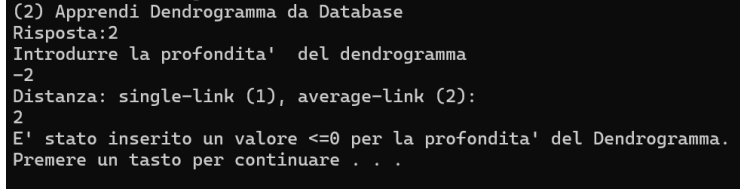
\includegraphics[width=\textwidth]{images/-2_valore_errato.png}
    \end{figure}

    L'inserimento di valori non ammissibili per il parametro di profondità (zero o negativi) viene rilevato dal sistema che, pur proseguendo con la richiesta del metodo di calcolo, interromperà l'elaborazione notificando l'anomalia.

\subsubsection{Controllo selezioni metodologiche} 
    
\begin{figure}[h!]
        \centering
        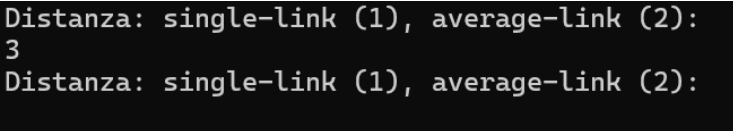
\includegraphics[width=\textwidth]{images/controllo_metodologie.png}
    \end{figure}
    L'inserimento di opzioni non valide per la selezione della metodologia di calcolo delle distanze viene gestito permettendo all'utente di riformulare la propria scelta.

\subsubsection{Verifica di compatibilità dimensionale} 
    \begin{figure}[h!]
        \centering
        \includegraphics[width=\textwidth]{images/compatibilità_dimensionale.png}
    \end{figure}
    Il sistema controlla la congruenza tra la cardinalità degli esempi nella tabella corrente e quella memorizzata nell'oggetto serializzato. In caso di incongruenza, viene visualizzato un messaggio esplicativo e l'esecuzione viene terminata.

\subsection{Gestione connettività client-server}
\begin{figure}[h!]
    \centering
    \includegraphics[width=\textwidth]{images/connettività_clientserver.png}
\end{figure}
L'avvio del client in assenza del componente server attivo genera un tentativo di connessione all'indirizzo locale (127.0.0.1) che, non trovando un endpoint disponibile, risulta in un rifiuto della connessione con relativa notifica.

\subsubsection{Elaborazione su dataset vuoti} 
    \begin{figure}[h!]
        \centering
        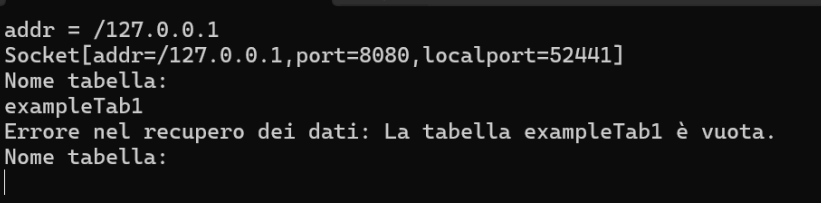
\includegraphics[width=\textwidth]{images/dataset_vuoti.png}
    \end{figure}

Quando l'utente tenta di eseguire un'analisi di clustering su una tabella priva di contenuti, il sistema identifica la condizione e fornisce un'appropriata segnalazione.

